\subsection{Controlled and natural occlusion}

We simulate occlusion by covering part of every annotated fruit with a
rectangular strip. This intervention adapts the region-erasing methods used for
augmentation and robustness testing \cite{devries2017cutout, zhong2020randomerasing} to a test-time setting
with a known hidden fraction, as used in controlled occlusion benchmarks
\cite{gilroy2023benchmark}. The strip enters each ground-truth box from a
randomly chosen side and covers a set fraction of its area. Thus, ``40\%
hidden'' has the same definition for a large fruit and a small one. We fill the
strip with a fruit-free background crop from the same image to preserve local
lighting and colour statistics. A flat black strip provides an appearance
control. The colour-directed variants cover either the redder or the greener
half. We select that half from the median $a^*$ along the axis with the greatest
colour separation. The ground-truth boxes continue to describe the full fruit.

We estimate natural overlap separately from intersections between untouched
ground-truth boxes. Because it omits leaves, this estimate is a lower bound on
total natural occlusion. It is also likely to overestimate fruit-on-fruit
coverage because rectangular boxes include background at their corners.

\begin{figure}[t]
  \centering
  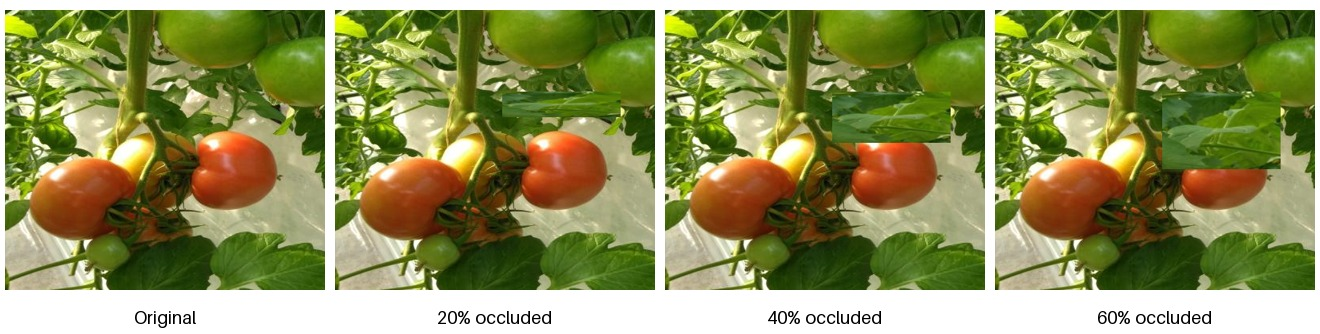
\includegraphics[width=\columnwidth]{occlusion_examples.jpg}
  \caption{Illustration of progressive synthetic occlusion on a representative
  red tomato: 0\%, 20\%, 40\%, and 60\% of its annotated box is covered from
  one side. The texture is sampled from a fruit-free region of the same frame.
  The straight boundary visualises the controlled intervention; quantitative
  results use the full evaluation set.}
  \label{fig:occlusion-examples}
\end{figure}
